\section{Aufgabe 1}

\subsection{Aufgabenbeschreibung}

Mit der Temperaturmessschaltung soll eine gemessene Spannung zur Steuerung einer zweistufigen Belüftungsanlage (hier simuliert durch zwei LEDs) verwendet werden. Bei einer bestimmten Temperatur soll zunächst der erste Lüfter, bei weiter steigender Temperatur ein zusätzlicher in Betrieb gehen. Hierfür ist es notwendig, sich zuerst über verschiedene Messschaltungen Gedanken zu machen, sowie sich über geeignete temperaturabhängige Bauteile zu informieren.

\subsection{Recherche zu Temperatursensoren}
\subsubsection{Arten von temperaturabhängigen Bauteilen}
Es gibt verschiedene Arten von temperaturabhängigen Bauteilen. Zwei spezielle Bauteile sind der PTC und der Supraleiter.\\
PTC heißt ausgeschrieben "`Positive Temperature Coefficient'' oder "`Kaltleiter''. Dabei steigt der elektrische Widerstand bei Erhöhung der Temperatur. Dabei gehört der PTC, wie auch der NTC zu den nichtlinearen Bauteilen.\\
Bei einem Supraleiter fällt der Widerstand nach dem Unterschreiten einer bestimmten Sprungtemperatur der elektrische Widerstand auf null ab.
\subsubsection{NTC}
Der NTC heißt ausgeschrieben "`Negative Temperature Coefficient'' oder auch "`Heißleiter''. Dabei sinkt der Widerstand mit steigender Temperatur.\\
NTC's werden aus keramischen Stoffen hergestllt, die auf Metalloxiden, wie die Oxide von Mangan, Nickel, Kobalt, Eisen, Kupfer, sowie Titan, basieren.

\paragraph{Vor-/Nachteile}

Als Vorteile von NTC's sind zu benennen: Eine kostengünstige Fertigung, kleine Baugrößen, lange Haltbarkeit, einfach austauschbar, Hochohmigkeit.\\
Dem gegenüber stehen die nicht-linearen Kennlinien weswegen ein Geeigneter Vorwiderstand zur Strombegrenzung notwendig ist, da der NTC ansonsten bei bestimmten Betriebstemperaturen durchbrennen könnte.

\paragraph{Einsatzgebiete}

NTC's werden als Temperatursensor, Einschaltstrom-Reduzierer, Sicherung und zur Temperaturstabilisierung von Halbleiterschaltungen verwedet.\\
Der typische Temperaturbereich in dem NTC's eingesetzt werden beträgt etwa -80°C bis +250°C.

\paragraph{Kennlinie}

\begin{figure}[h!]
	\centering
	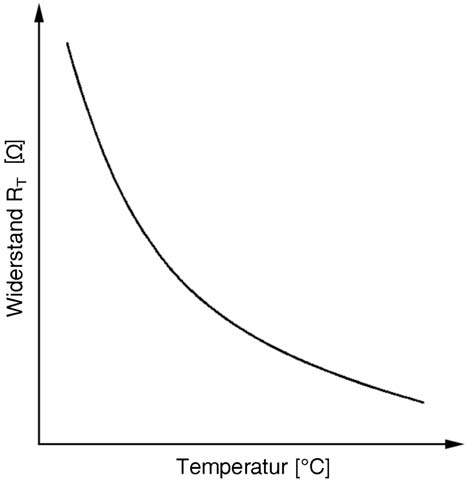
\includegraphics[scale=0.7]{pics/ntc-kennlinie.jpg}
	\caption{Kennlinie eines NTC's mit dem Widerstand aufgetragen zur Umgebungstemperatur}
	\label{fig:ntc}
\end{figure}

Die Kennlinie eines NTC's lässt sich in der Abbildung \ref{fig:ntc} auf Seite \pageref{fig:ntc} betrachten.\\
Man kann die Kennlinie aber auch als Gleichung Gleichung in der Form: 

\begin{align}
R(T) = R_{ref}\cdot e^{(A+\frac{B}{T} + \frac{C}{T^2} + \frac{D}{T^3})}
\end{align}
\footnote{Dem Datenblatt des ausgeteilten NTC's auf Seite 4 entnommen.}

darstellen. Dabei sind A,B,C und D materialabhängige Konstanten. \(R_{ref}\) stellt den Widerstand bei einer bestimmten Referenztemperatur (meist 25°C) dar.


\subsection{L"ufterschaltung}

\subsubsection{Dimensionierung der Messschaltung}

Für die Dimensionierung der Messschaltung müssen zunächst Überlegungen angestellt werden, unter welchen Randbedingungen die Messschaltung betrieben wird.\\
Es wird angenommen, dass die Belüftungsanlage zur Belüftung eines Gebäudes oder Raumes verwendet wird. Dadurch ergeben sich Temperaturen von etwa 10°C bis etwa 45°C. Als Extremfall sollen 0°C und 55°C angenommen werden.\\
Dem Datenblatt des eingesetzten NTCs entnommen kann der NTC im Bereich zwischen 0°C und 55°C 100\% der Maximalleistung von \(P_{max} =\) 500mW vertragen.\\
Die Widerstände \(R_T\) des NTCs bei verschiedenen Temperaturen T können dem Datenblatt des NTCs entnommen werden.
\begin{align}
bei\ T&=\ 0^{\circ} C:\ &I_{max1} &= \sqrt{\frac{P_{max}}{R_0}} &= \sqrt{\frac{500mW}{325k\Omega}} &= 3,92mA\\
bei\ T&=\ 55^{\circ} C:\ &I_{max2} &= \sqrt{\frac{P_{max}}{R_{55}}} &= \sqrt{\frac{500mW}{3k\Omega}} &= 12,9mA 
\end{align}

Um zu überprüfen ob der Widerstand im Spannungsteiler eine Mindestgröße benötigt, wird berechnet welcher Strom durch den NTC bei T=0°C bzw. T=55°C abfällt wenn kein Widerstand verwendet wird.\\

\begin{align}
&I_0 &=\frac{U_0}{R_0}&=\frac{10V}{32,5k\Omega}&=0,3mA
\\&I_{55} &=\frac{U_0}{R_{55}}&=\frac{10V}{3k\Omega}&=3,3mA
\end{align}

Das heisst: Bei jedem beliebigen Widerstand R, im gültigen Arbeitsbereich zwischen T=0°C und T=55°C, fliesst nicht genügend Strom um den NTC über seine Leistungsgrenze zu belasten.
Der Widerstand R ist somit für die Anwendung frei wählbar.

Für die Anwendung wird angenommen, dass der erste Lüfter bei einer Temperatur von etwa 30°C schalten soll. Für diese Temperatur hat der NTC einen Widerstand von \(R_{30} = 8059 \Omega\) für R ergibt sich dann mit der Spannungsteilerregel:
\begin{align}
R=\frac{U_R}{U_0-U_R}\cdot R_{30} = \frac{0,7V}{10V-0,7V}\cdot 8059\Omega \approx 600\Omega \label{eqn:temp}
\end{align}

Die maximale bzw. minimale Spannung über R beträgt mit der Wahl von R:

\begin{align}
U_{R_{max}} = \frac{R}{R_{55}+R}\cdot U_0 = \frac{600\Omega}{2989\Omega + 600\Omega}\cdot 10V = 1,67V\\
U_{R_{min}} = \frac{R}{R_{0}+R}\cdot U_0 = \frac{600\Omega}{32500\Omega + 600\Omega}\cdot 10V = 0,18V
\end{align}

\subsubsection{Aufbau der Messschaltung}

\paragraph{Berechnungen und theoretische Überlegungen}
Den Schaltzeitpunkt der ersten LED/des ersten Lüfters kann durch einen Transistor in Emitterschaltung erfolgen, da der bipolare Transistor ab einer Basis-Emitter-Spannung von 0,7V die Kollektor-Emitter-Diode durchschaltet.\\
Die Basisstrombegrenzung lässt sich mit einem \(1k\Omega\) Widerstand vor der Basis verwirklichen. So fließt nur unwesentlich Strom in die Basis ab und der Spannungsteiler wird nicht stark belastet.\\

Die zweite Stufe mit der zweiten LED/des zweiten Lüfters kann durch einen zweiten Transistor in Emitterschaltung und zusätzlicher Diode am Emitter realisiert werden. Ein Vorwiderstand an der Basis zur Basisstrombegrenzung muss auch eingesetzt werden.\\
Durch die Diode am Emitter wird der benötigte Spannungsabfall über der Basis-Emitter des zweiten Transistors auf 1,4V erhöht. Dadurch kann der Schaltzeitpunkt der zweiten LED auch eingestellt werden.

\paragraph{Simulation in LTSpice}

Wie in Abbildung \ref{fig:ntc-spice} auf Seite \pageref{fig:ntc-spice} zu sehen ist wurde die Schaltung in LTSpice aufgebaut, statt den Leuchtdioden wurden einfache Dioden verwendet.\\

\begin{figure}[h!]
	\centering
	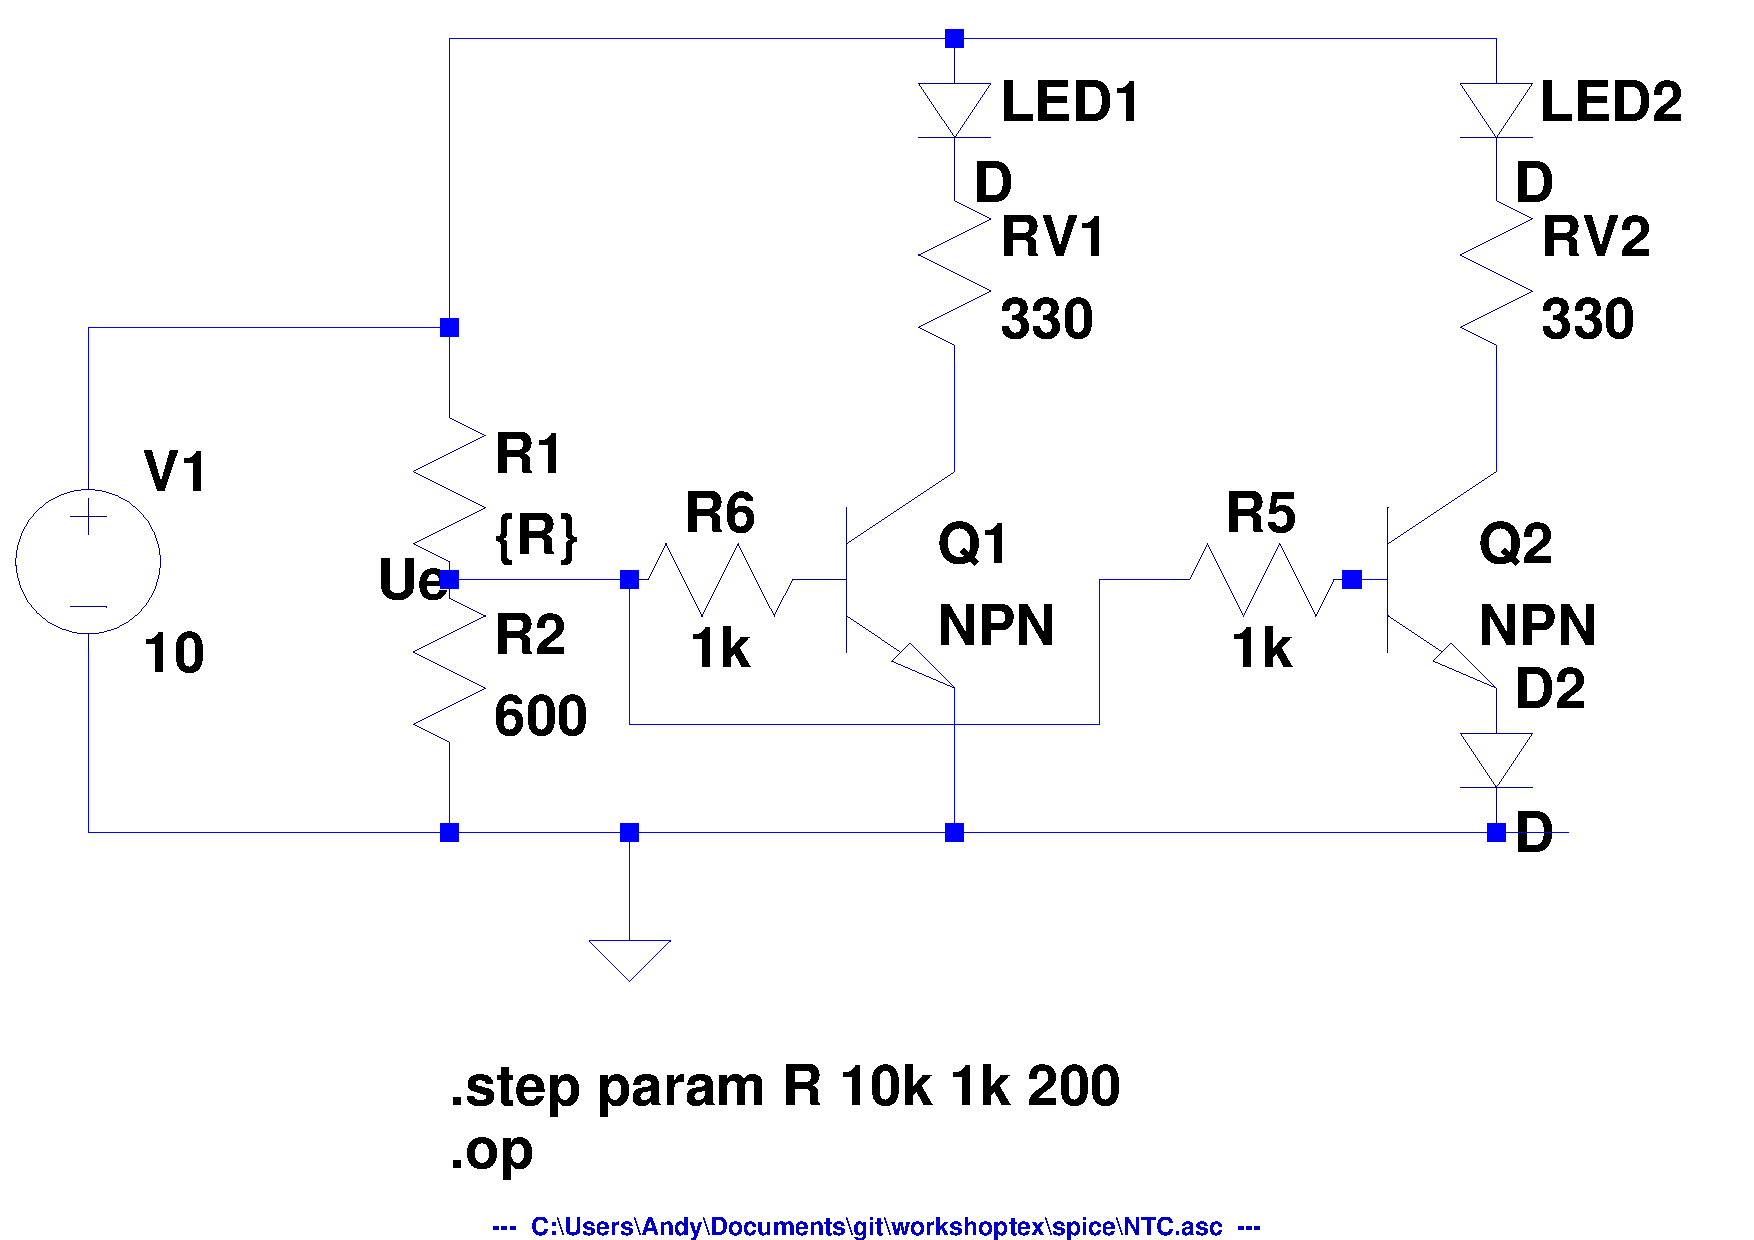
\includegraphics[scale=0.4]{pics/NTC-Circuit}
	\caption{Aufbau der Messschaltung in LTSpice}
	\label{fig:ntc-spice}
\end{figure}

Die Simulation wurde mit Blick auf den NTC und dem abnehmenden Widerstand im Verlauf der Erhitzung durchgeführt. In Abbildung \ref{fig:ntc-simu} auf Seite \pageref{fig:ntc-simu} ist das passende Diagramm zu sehen.\\
Auf der X-Achse ist dabei die Spannung \(U_R\) über dem Widerstand R aufgetragen. In Y-Richtung ist der Kollektor-Strom durch die LED's aufgetragen. Dem Diagramm ist zu entnehmen, dass die erste LED ab etwa 0,7V über dem Widerstand R zu leiten beginnt und die zweite LED etwa ab 1,4V über dem Widerstand R leitet.

\begin{figure}[h!]
	\centering
	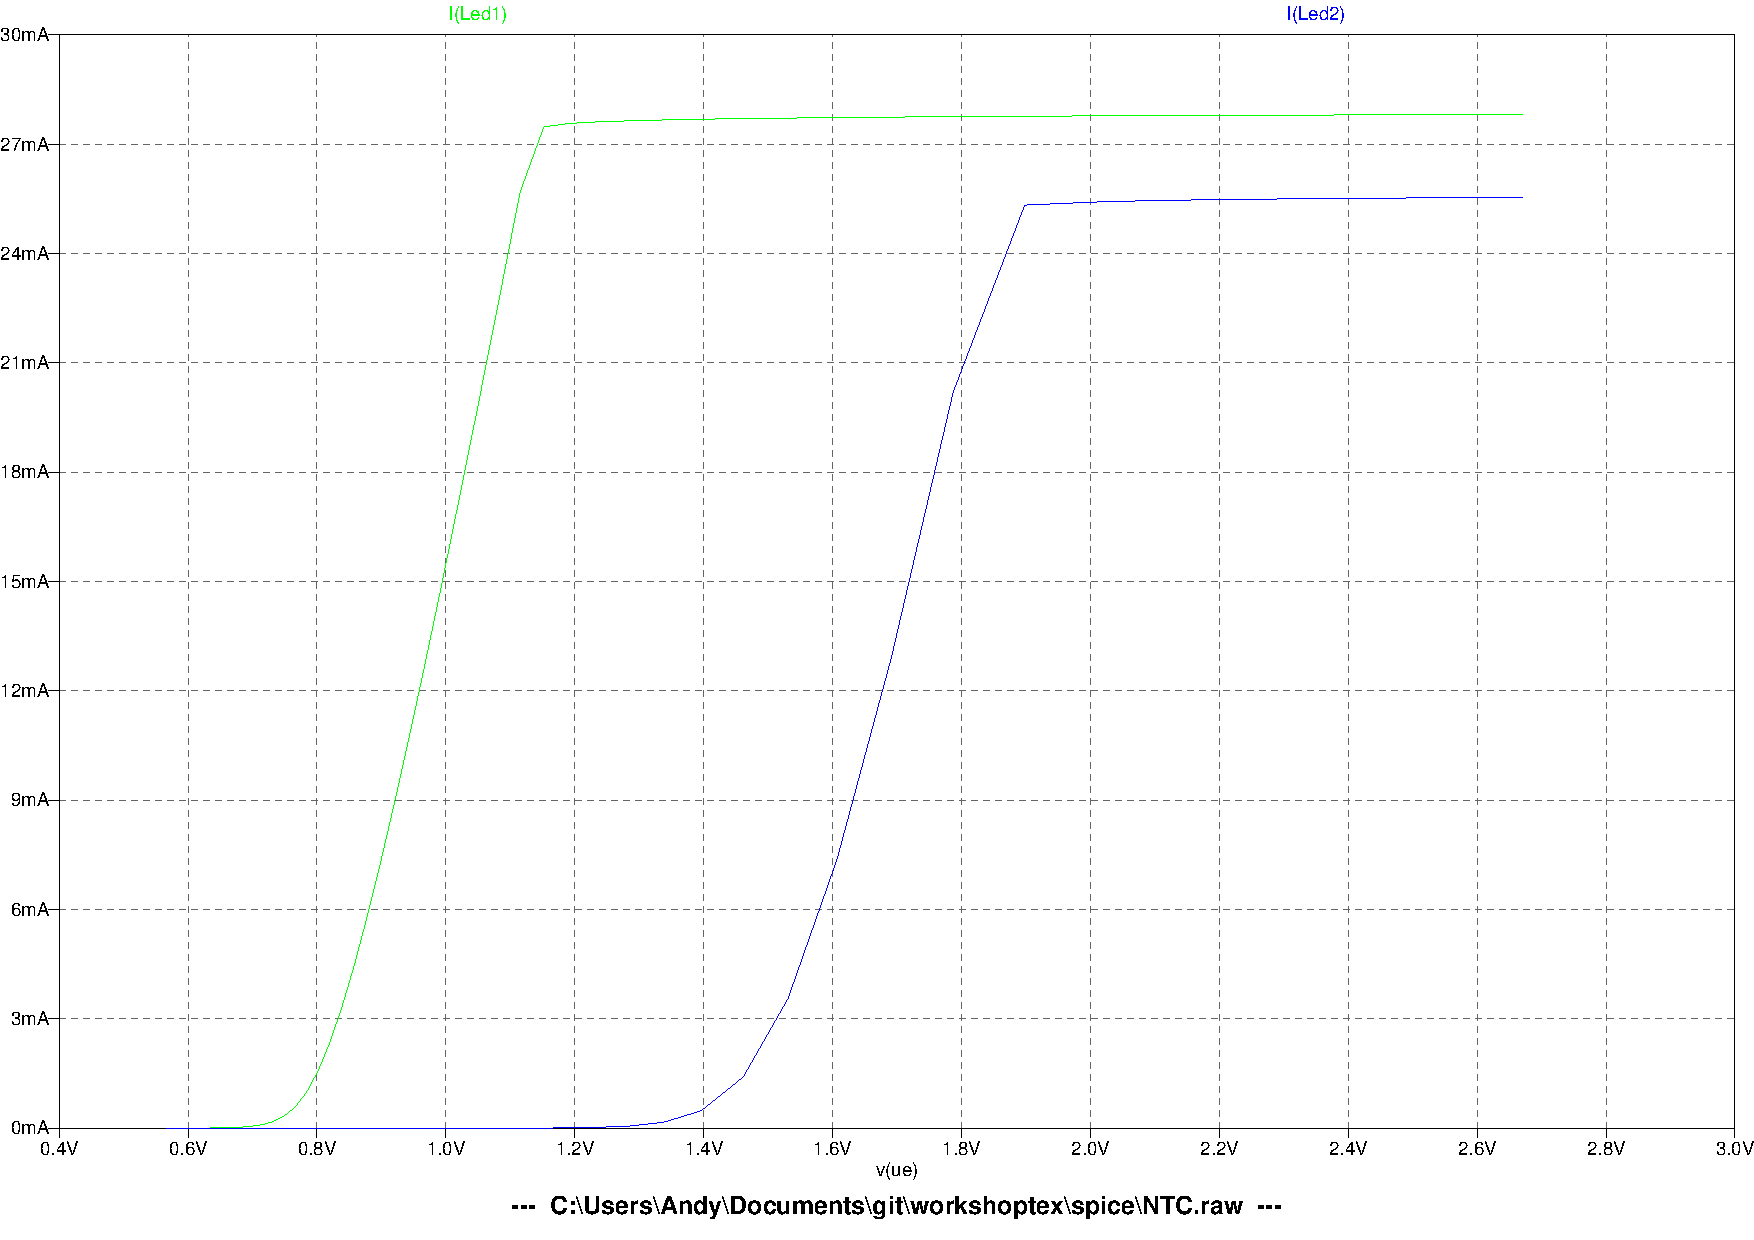
\includegraphics[scale=0.4]{pics/NTC-Diagramm}
	\caption{Simulation der Messschaltung}
	\label{fig:ntc-simu}
\end{figure}

\paragraph{Aufbau der Messschaltung auf dem EI-Board}

Mit erfolgreicher Simulation wird die Schaltung auf dem EI-Board aufgebaut. In Abbildung \ref{fig:ntc-aufbau} auf Seite \pageref{fig:ntc-aufbau} ist der Aufbau zu sehen. Bei einer ersten Messung ist jedoch aufgefallen, dass der Widerstand R für die Messung mit \(600\Omega\) zu hoch gewählt wurde. Die erste LED leuchtet in der Realität bei einem Widerstand von \(600\Omega\) schon bei Raumtemperatur. Deshalb wurde der nächstkleinere Widerstand mit dem Wert \(470\Omega\) für die weiteren Versuche verwendet.\\

\begin{figure}[h!]
	\centering
	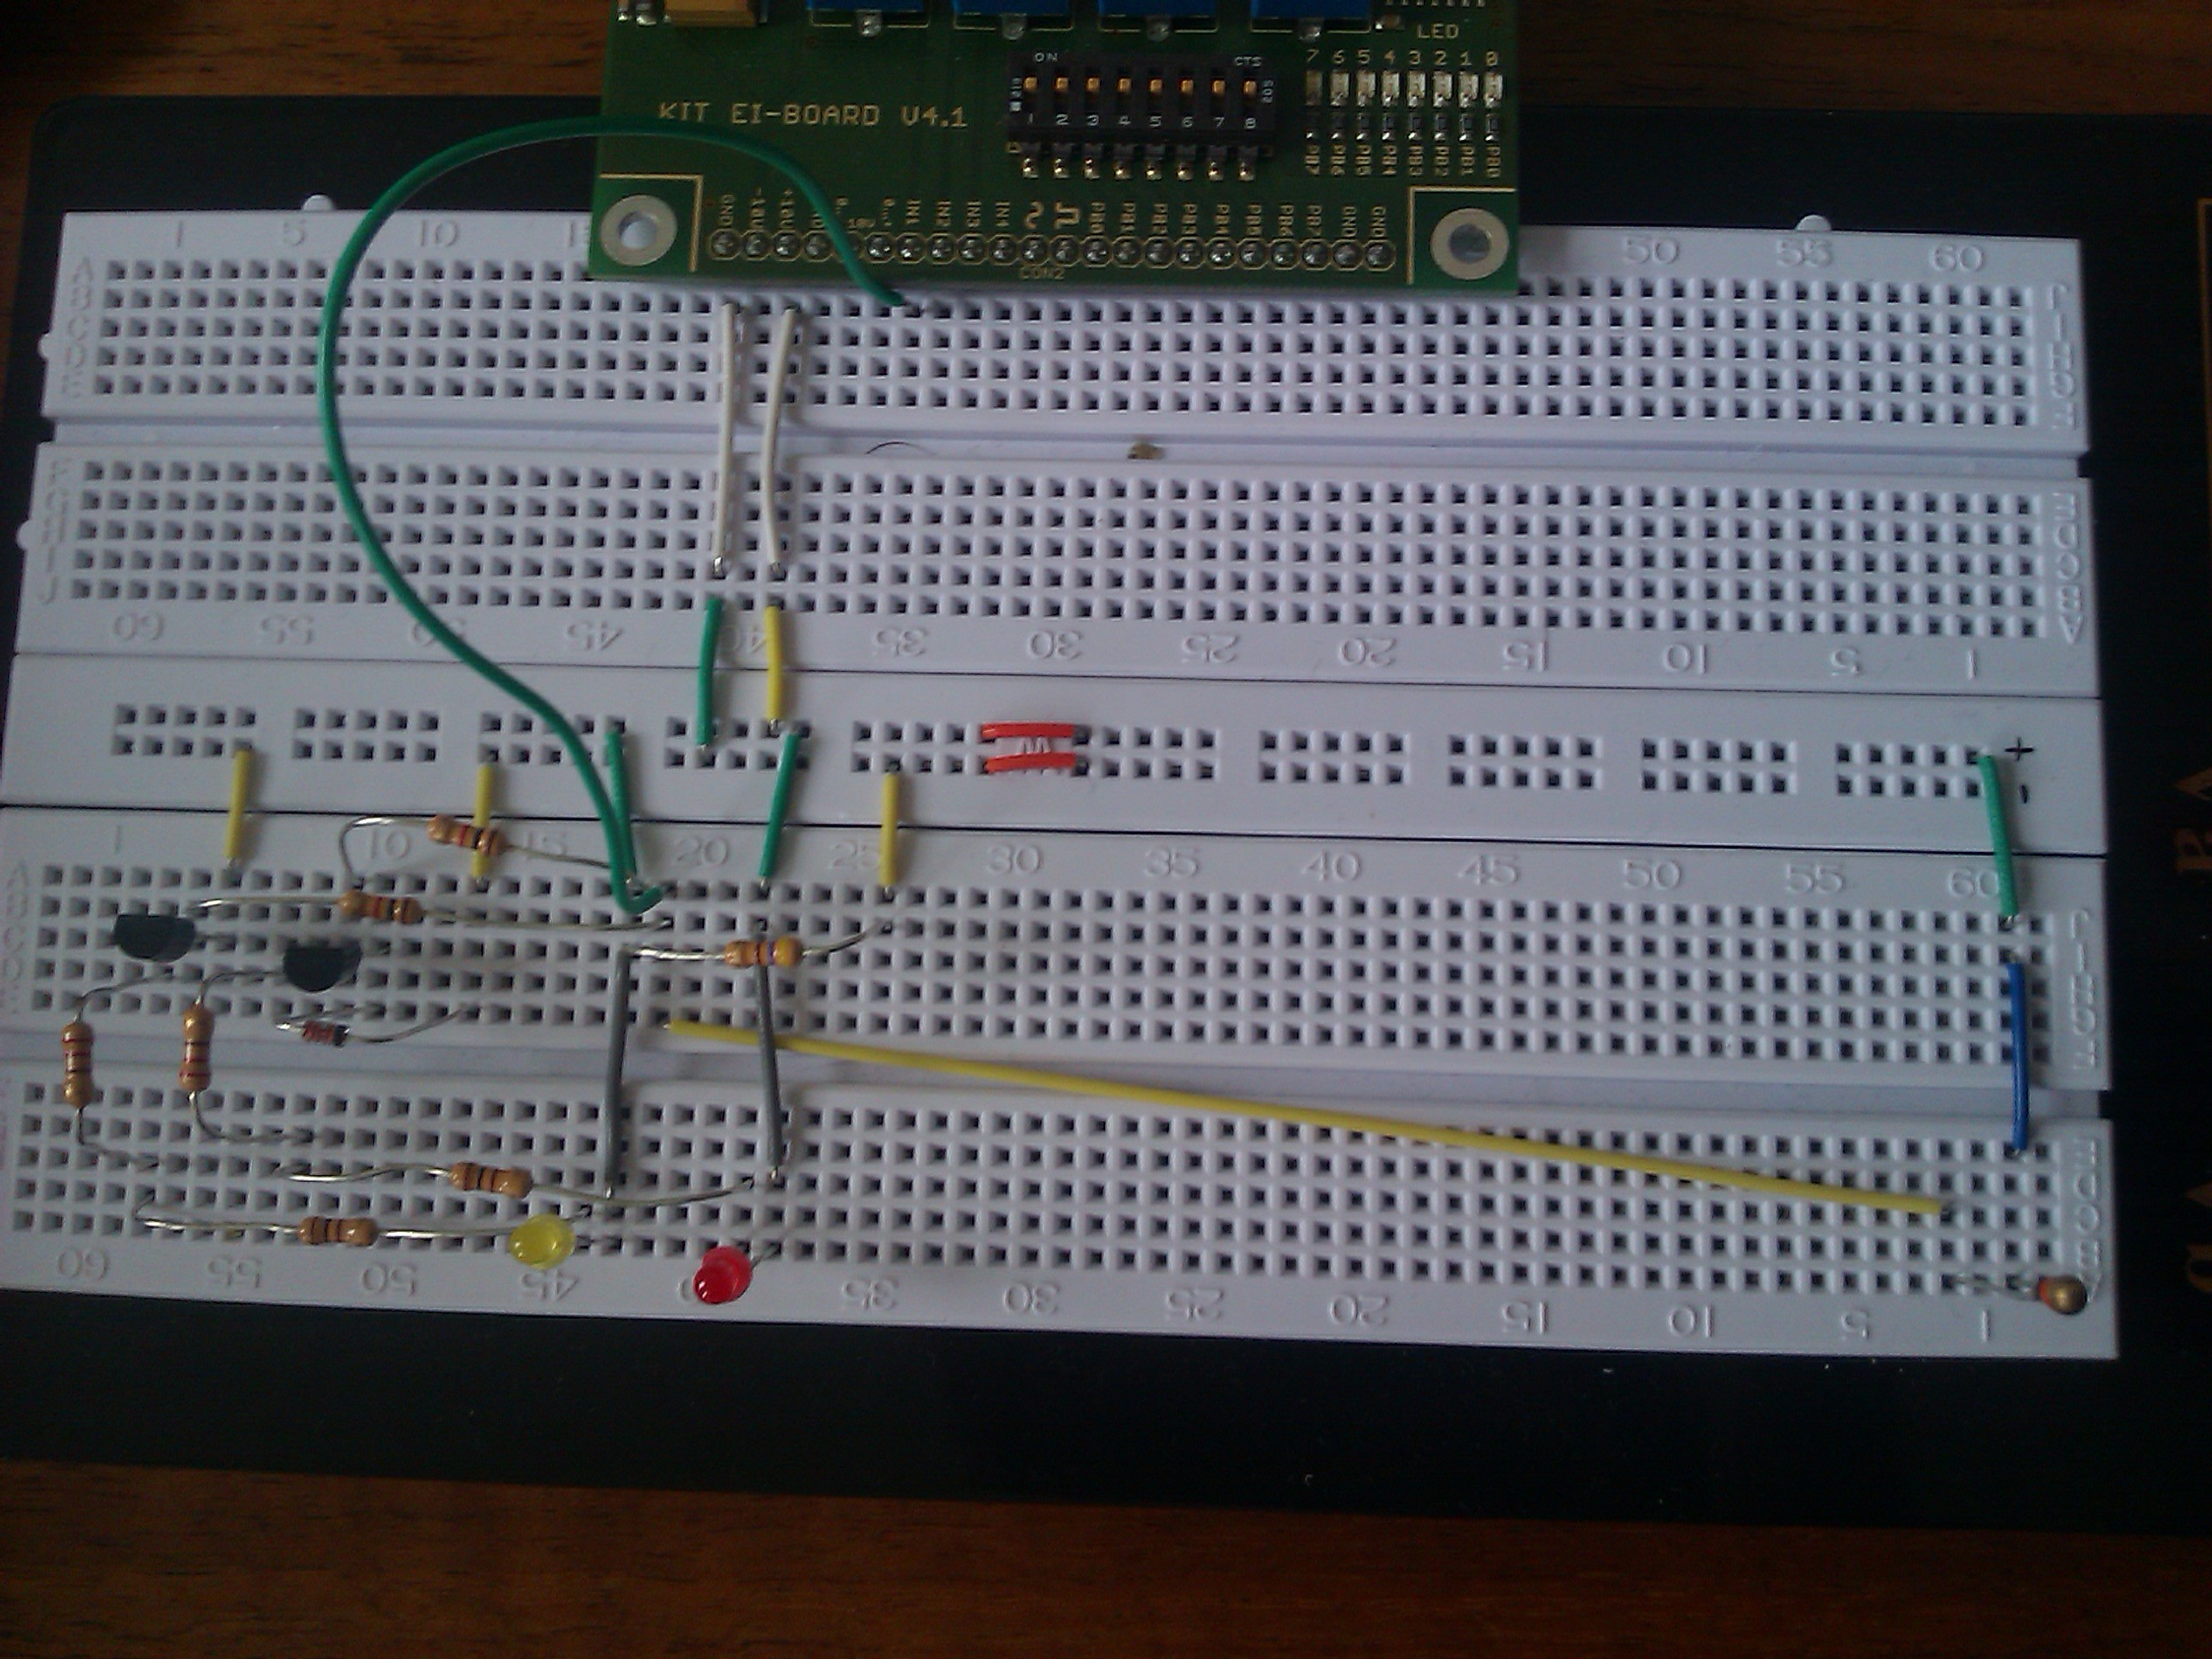
\includegraphics[scale=0.2]{pics/ntc-aufbau.jpg}
	\caption{Aufbau der Messschaltung auf dem EI-Board}
	\label{fig:ntc-aufbau}
\end{figure}

Nach kurzer Erwärmung mit dem Feuerzeug beginnt die erste LED zu leuchten. (Abb. \ref{fig:ntc-led1} S. \pageref{fig:ntc-led1})\\
Bei weiterer Erwärmung leuchten beide LED's.(Abb. \ref{fig:ntc-led2} S. \pageref{fig:ntc-led2})\\ 

\begin{figure}[h!]
	\centering
	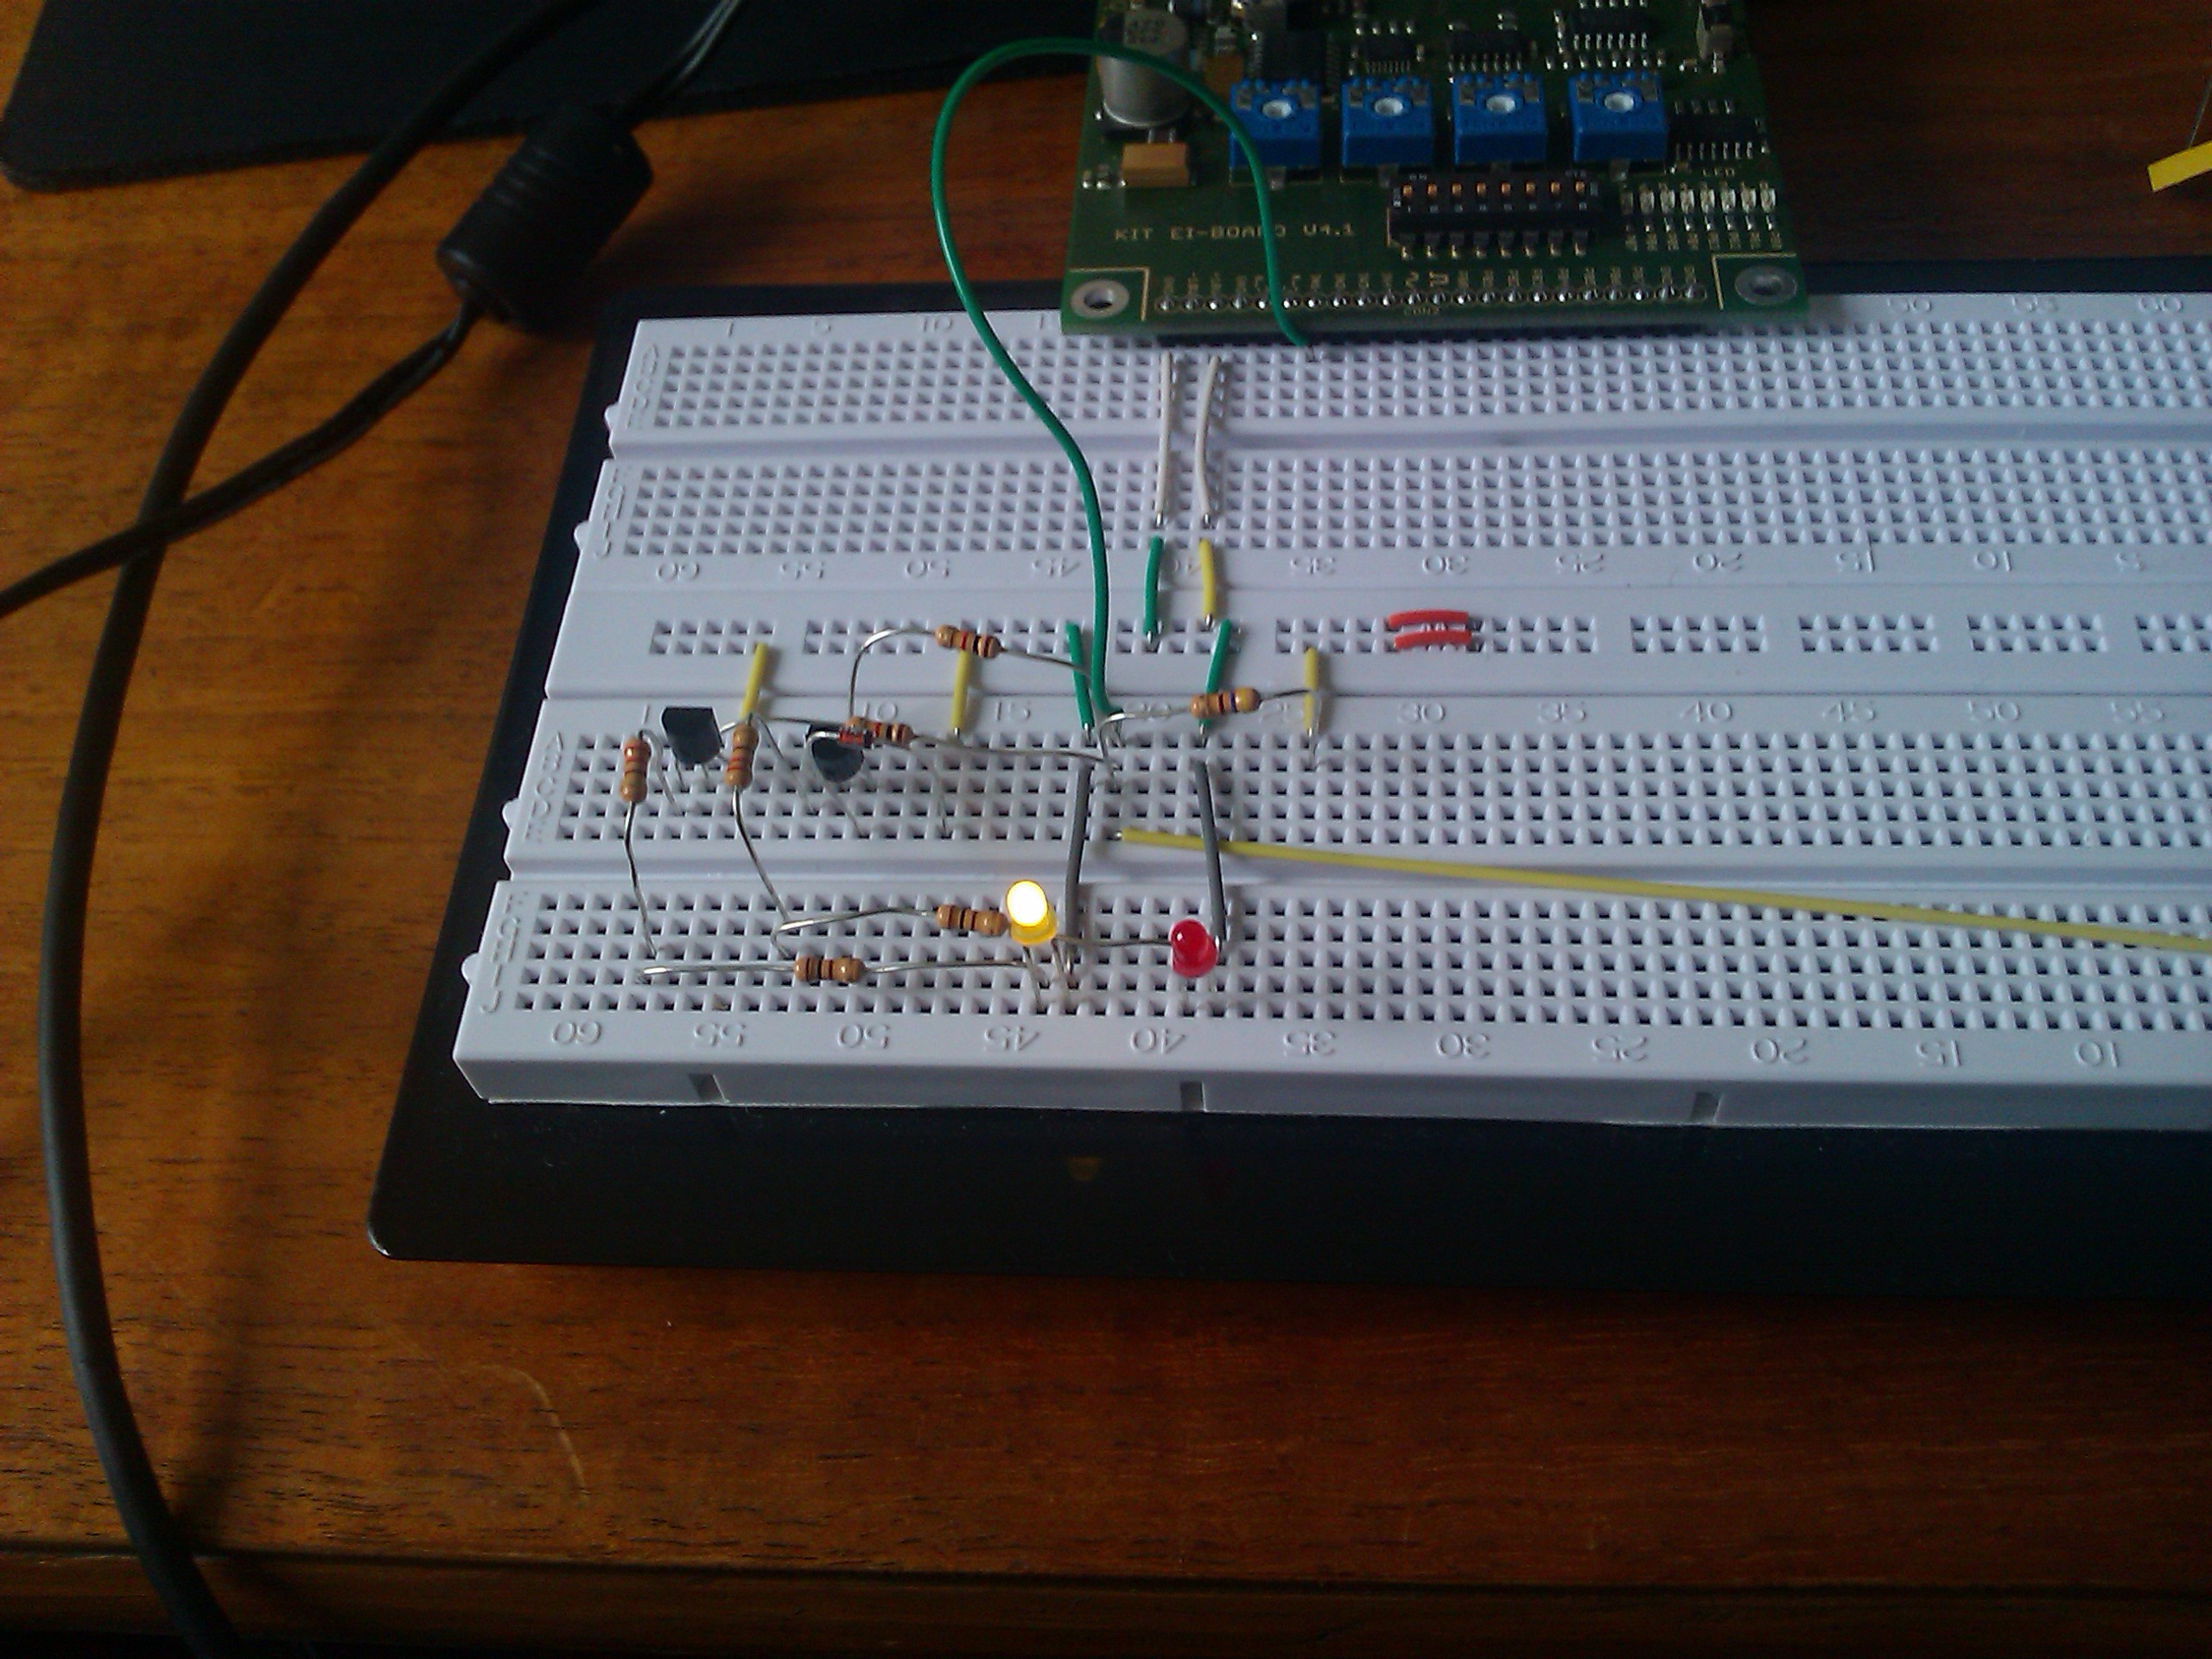
\includegraphics[scale=0.2]{pics/ntc-led1.jpg}
	\caption{Die erste LED leuchtet}
	\label{fig:ntc-led1}
\end{figure}

\begin{figure}[h!]
	\centering
	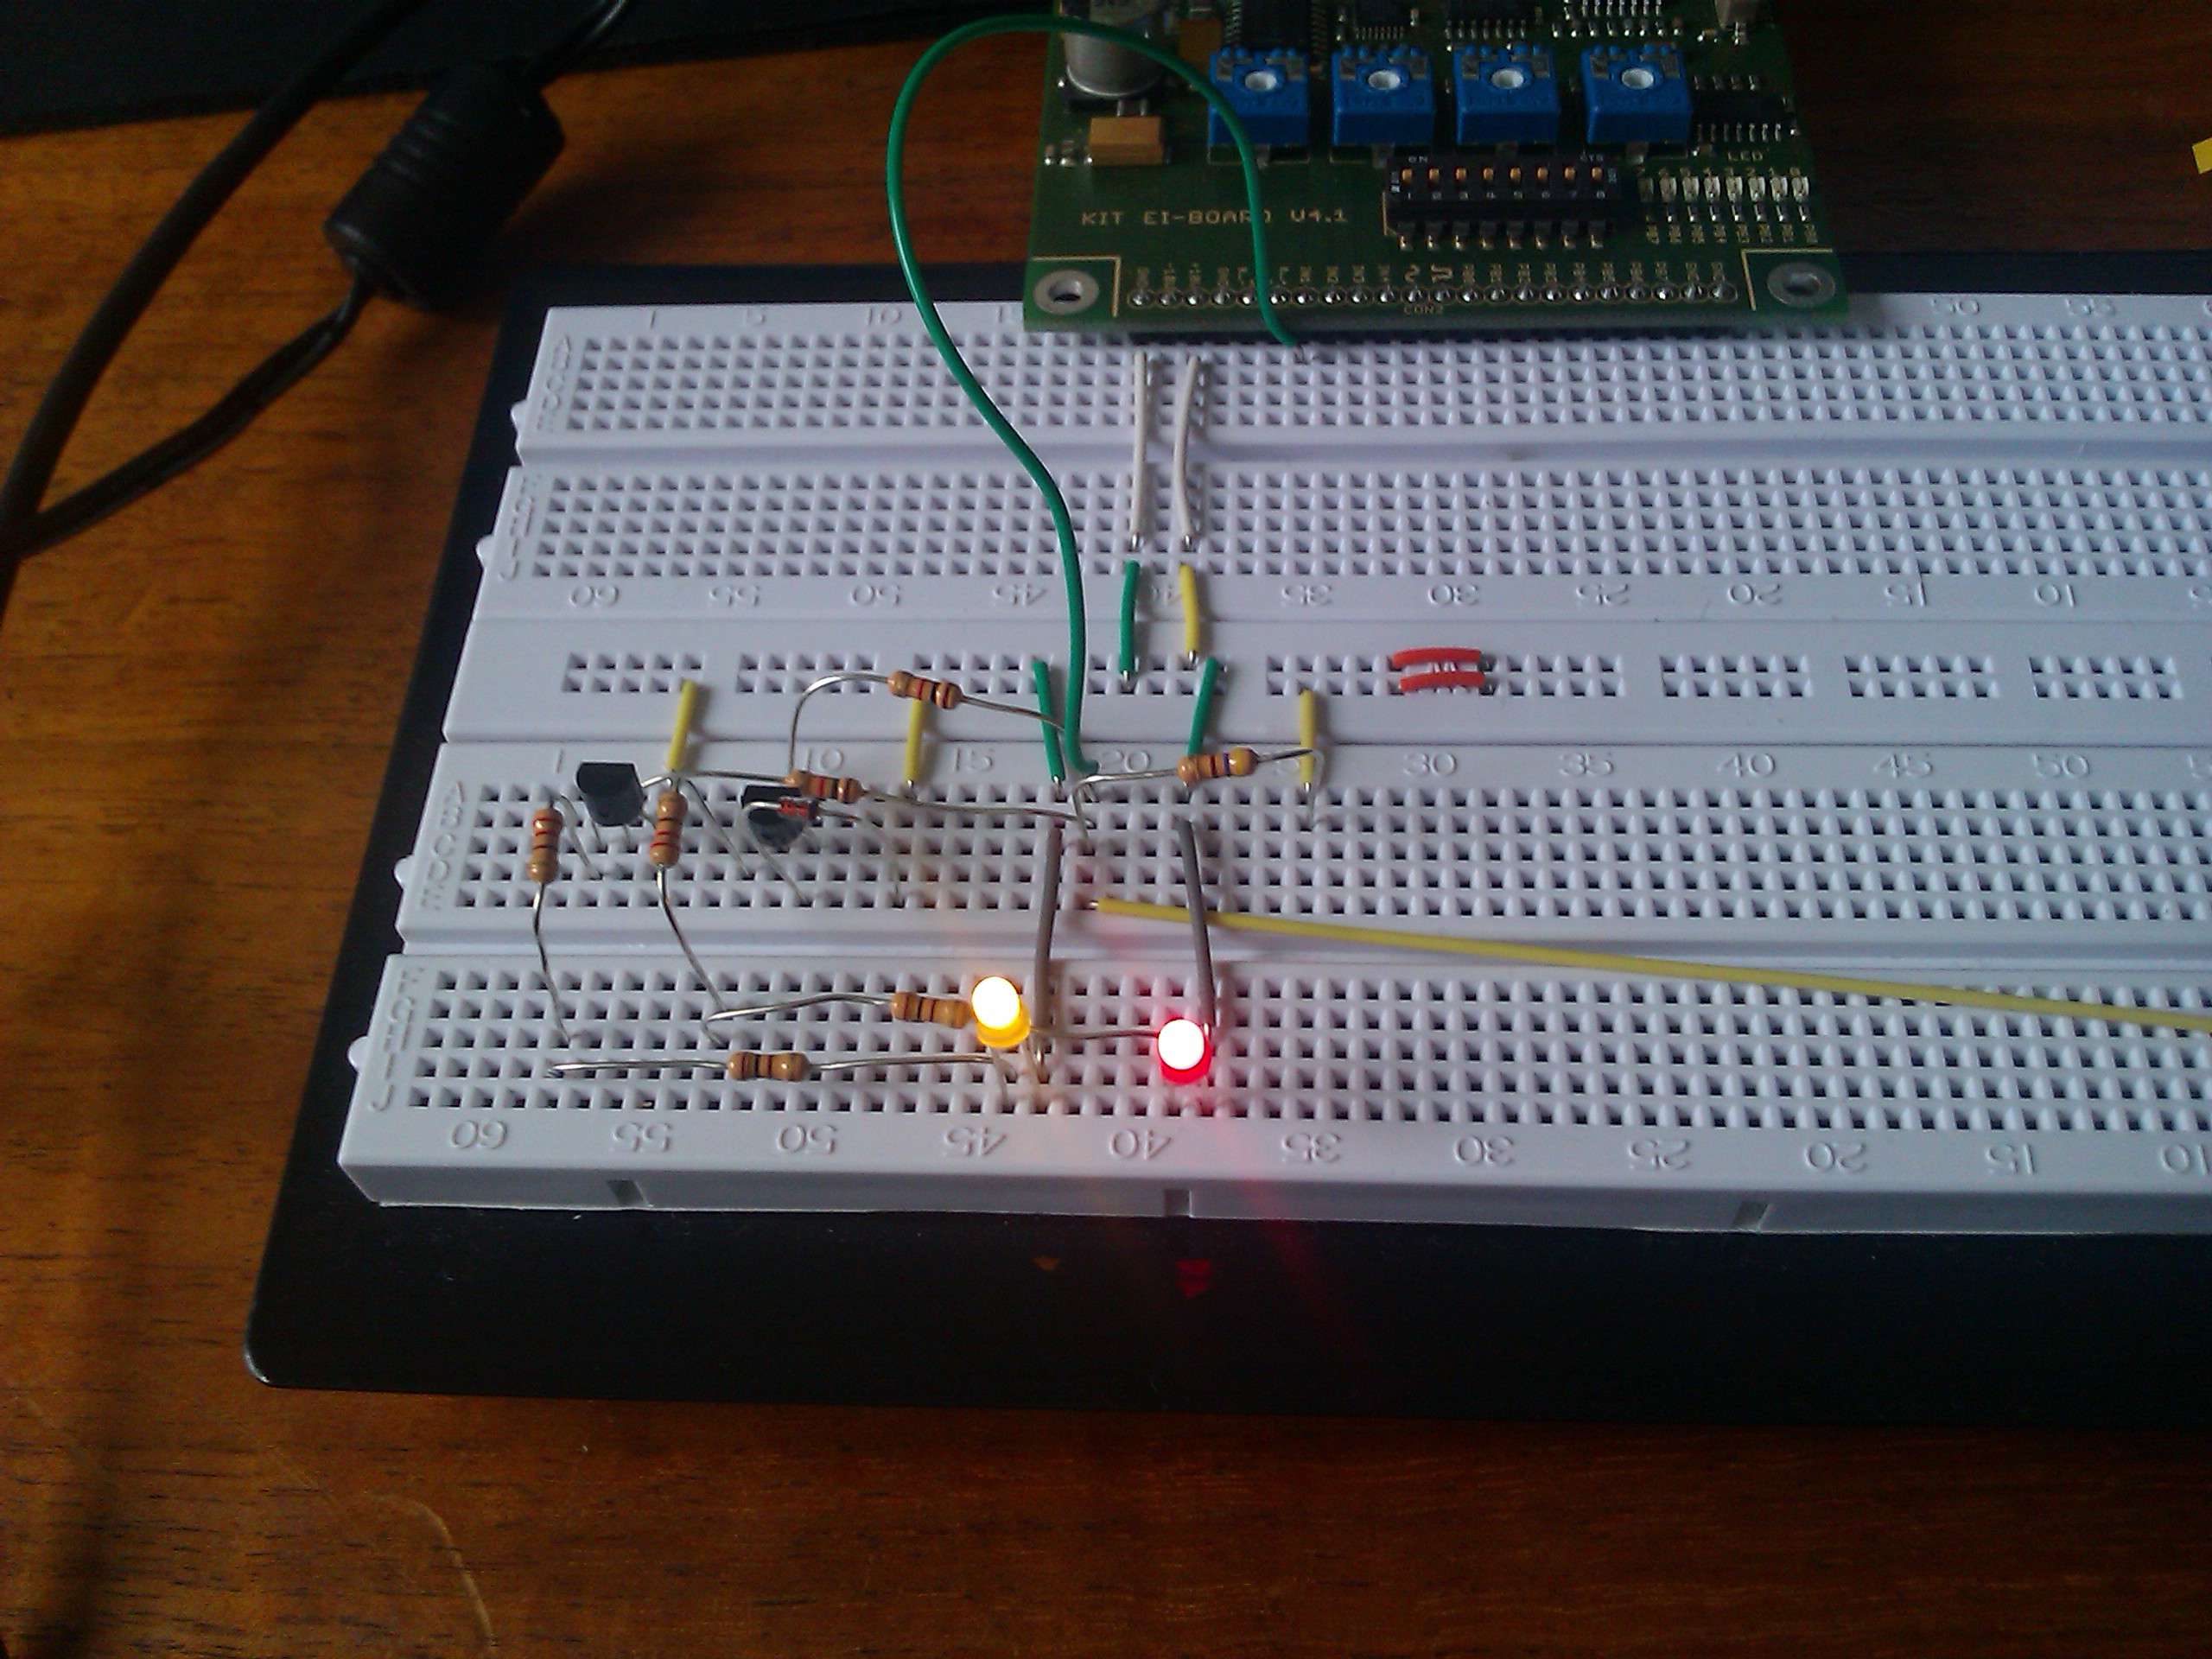
\includegraphics[scale=0.2]{pics/ntc-led2.jpg}
	\caption{Beide LED's leuchten}
	\label{fig:ntc-led2}
\end{figure}

\paragraph{Schaltzeitpunkt der Transistoren}

Der Schaltzeitpunkt bei bestimmten Temperaturen lässt sich mit einer Spannungsmessung über dem Widerstand R verifizieren. Bei einem Widerstand R von \(470\Omega\) hat der erste Transistor bei etwa 0,7V und der zweite Transistor bei etwa 1,4V Spannung über dem Widerstand R geschaltet. 
Mithilfe der Gleichung \ref{eqn:temp} auf Seite \pageref{eqn:temp} lässt sich nun die Temperatur der Schaltzeitpunkte bestimmen.\\
Durch Umstellen der Gleichung erhält man für \(R_{T_1} = 6200\Omega\) und für \(R_{T_2} = 2800\Omega\). Dem Datenblatt lässt sich dann entnehmen, dass die Temperaturen \(T_1\) bzw. \(T_2\) der Schaltzeitpunkte etwa bei 37°C bzw. 57°C liegen.

\subsection{Zusammenfassung}

